% !TEX encoding   = UTF8
% !TEX spellcheck = ru_RU
% !TEX root = ../seminars.tex

%%================================
\chapter{Вентили и булева алгебра}
%%================================

%%======================================
\section{Многоуровневая организация ЭВМ}
%%======================================
\begin{center}
  \begin{tikzpicture}[node/.style={rectangle, draw, thick, dashed, inner ysep=1mm},
                      arrow/.style={line width=1pt, dashed,
                                    arrows={-Latex[width=1pt 3, length=10pt]}}]
    \node (C)[node] {язык C};
    \node (asm)[node, below=5mm of C] {язык ассемблера};
    \node (hardware)[node, below=9mm of asm, label=right:<<железо>>] {аппаратное обеспечение};

    \draw[->,arrow] (C) -- (asm);
    \draw[->,arrow] (asm) -- node[right] {\ldots} (hardware);
  \end{tikzpicture}
\end{center}



%%==================
\subsection{Вентили}
%%==================
\begin{center}
  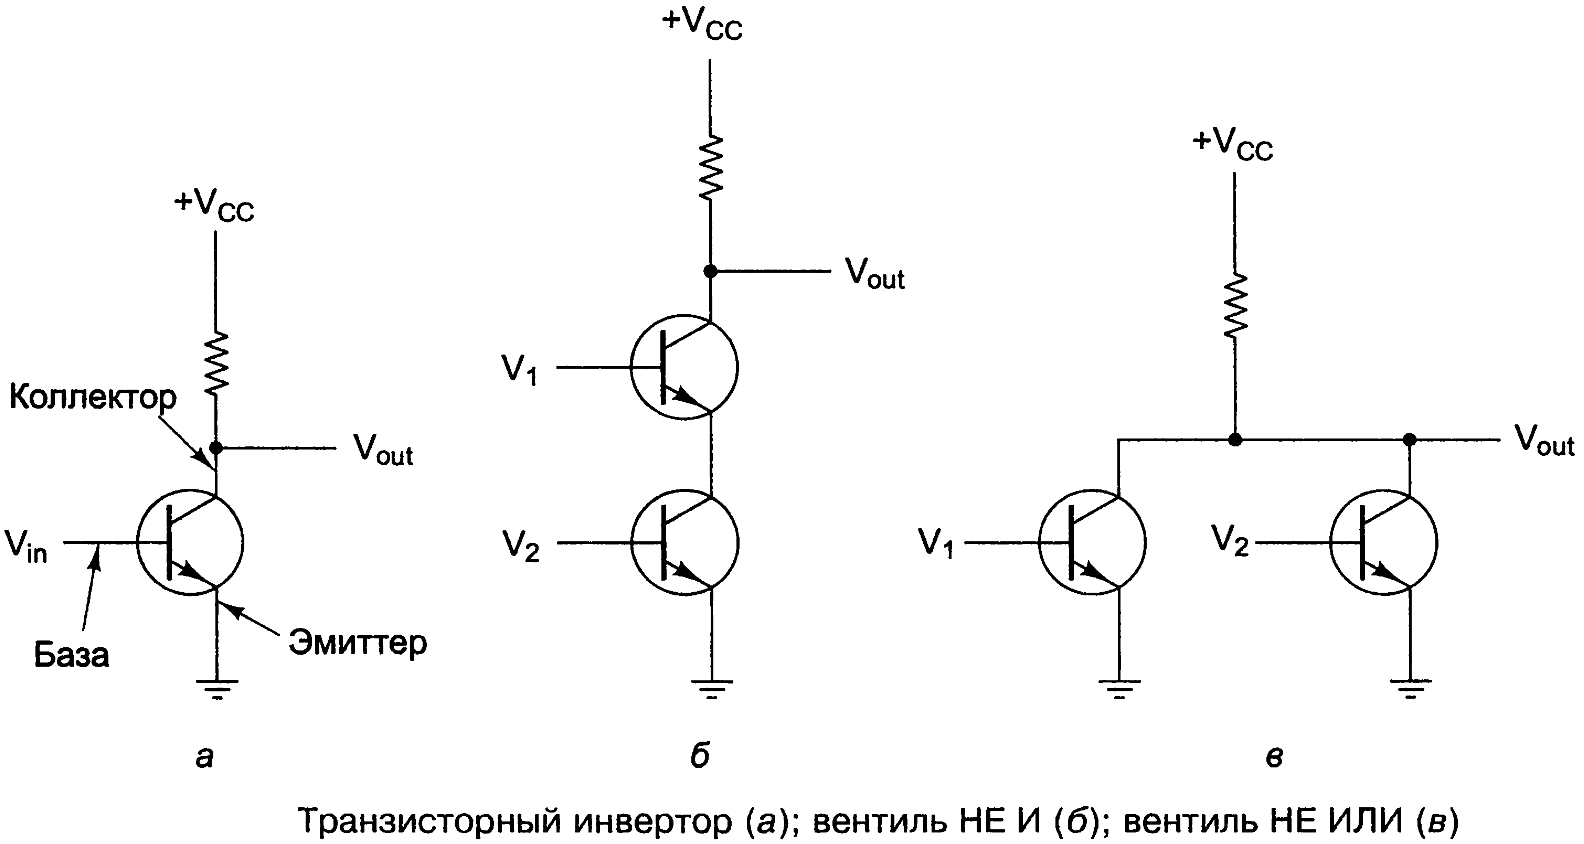
\includegraphics[width=0.8\columnwidth]{images/transistors.png}
\end{center}

\emph{Цифровая схема}~--- это схема, в которой есть только два логических значения:~\code{0} или \code{ложь} (сигнал от~0 до 1\,В) и~\code{1} или \code{истина} (сигнал от~2 до 5\,В).

\emph{Вентили}~--- это электронные устройства, которые позволяют получать различные функции от цифровых (двузначных: \code{0} или \code{1}) сигналов. Вентили лежат в основе аппаратного обеспечения, на котором строятся все цифровые компьютеры.

\begin{center}
  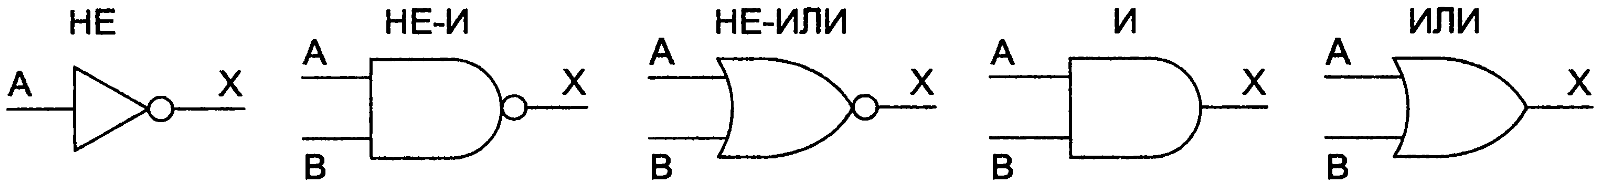
\includegraphics[width=0.8\columnwidth]{images/gates.png}
\end{center}



%%======================
\section{Булевы функции}
%%======================
\emph{Алгебра релейных схем}, \emph{булева функция \(n\) переменных}, \emph{\(2^n\) значений}, \emph{таблица истинности}.

Пример: \(M = f(A,B,C)\)~--- функция большинства, которая принимает 0, если большинство переменных равны 0, и 1, если большинство переменных равны 1.

\begin{center}
\textbf{СДНФ} \(=\) Совершенная Дизъюнктивная Нормальная Форма
\end{center}
\[
  M = \bar ABC + A\bar BC + AB\bar C + ABC
\]

\begin{enumerate}
\item Составить таблицу истинности.
\item Включить инверторы для каждого входного сигнала.
\item Нарисовать вентиль \code{И} для строк таблицы со значением 1.
\item Соединить вентили \code{И} с соответствующими входными сигналами.
\item Вывести выходы всех вентилей \code{И} и направить на вход вентиля \code{ИЛИ}.
\end{enumerate}

\medskip
Любую булеву функцию можно реализовать при помощи вентилей \code{НЕ}, \code{И} и \code{ИЛИ}.



%%================
\WhatToReadSection
%%================
\begin{tabular}{@{}l@{}}
  \citeauthor[глава~1, стр.~2--23, 50--106]{Harris:2015:ru} \\
  \citeauthor[глава~1, стр.~20--26; глава~3, стр.~172--182]{Tanenbaum:2013:ru}
\end{tabular}



%%===============
\ExercisesSection
%%===============
\begin{exercise}
\item Постройте схему для вычисления булевой функции \code{ИСКЛЮЧАЮЩЕЕ-ИЛИ} (\code{XOR}).

\item Реализуйте вентили \code{НЕ}, \code{И} и \code{ИЛИ} на основе \underline{только} вентилей \code{НЕ-ИЛИ}.

\item Реализуйте вентили \code{НЕ}, \code{И} и \code{ИЛИ} на основе \underline{только} вентилей \code{НЕ-И}.

\item Докажите эквивалентность следующих схем
\begin{center}
  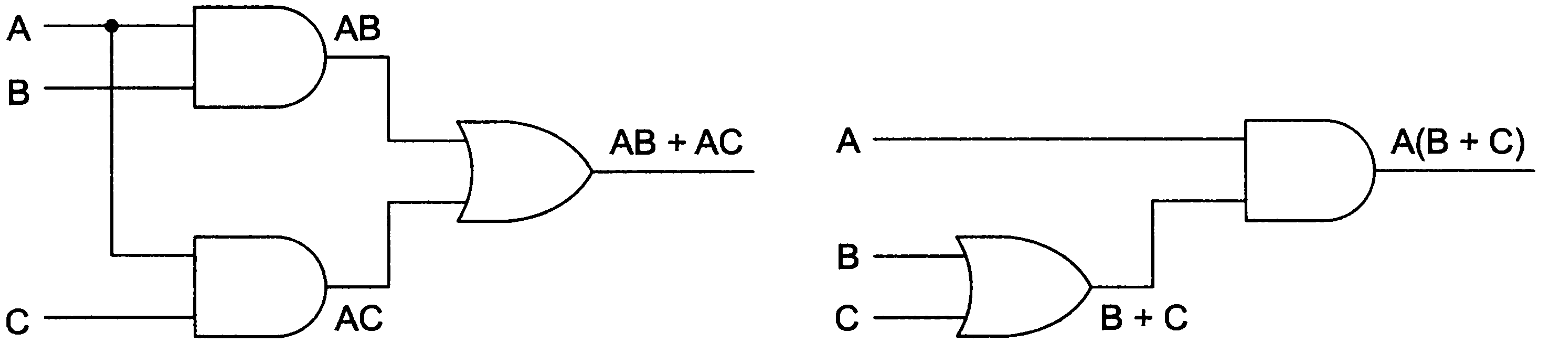
\includegraphics[width=0.8\columnwidth]{images/ex_eq_gates.png}
\end{center}

\end{exercise}
